\documentclass{article}
\usepackage[english]{babel}
\usepackage[utf8]{inputenc}
\usepackage{fancyhdr}
\usepackage{amsmath}
\usepackage{amsfonts}
\usepackage{mathrsfs}
\usepackage{mathtools}
\usepackage{indentfirst}
\usepackage{hyperref}
\usepackage{tikz,amsmath}
\usepackage{tikz,tkz-tab,amsmath}
\usetikzlibrary{trees}
\usetikzlibrary{arrows}
\usepackage{cancel}
\usepackage{xfrac}  

\usepackage{enumerate}

%\setlength{\TPHorizModule}{1mm}
%\setlength{\TPVertModule}{1mm}
  
% to disable automatic indentation on new paragraphs
%\setlength{\parindent}{0pt}

\hypersetup{
    colorlinks=true,
    linkcolor=blue,
    filecolor=magenta,
    urlcolor=blue,
}
\urlstyle{same}

\parskip 1ex

\usepackage{geometry}
 \geometry{
 a4paper,
 left=20mm,
 top=20mm,
 bottom=20mm,
 right=20mm
 }
\usepackage{multicol}
\pagestyle{fancy}
\fancyhf{}
\lhead{Matthieu Bessat}
\rhead{DM 9 - 14 dec. 2020}
\rfoot{Page \thepage}

\makeatletter
\def\@seccntformat#1{%
  \expandafter\ifx\csname c@#1\endcsname\c@section\else
  \csname the#1\endcsname\quad
  \fi}
\makeatother

\makeatletter
\renewcommand*\env@matrix[1][*\c@MaxMatrixCols c]{%
  \hskip -\arraycolsep
  \let\@ifnextchar\new@ifnextchar
  \array{#1}}
\makeatother

\newcommand{\vspacem}{\vspace{3mm}}
\newcommand{\bfrac}[2]{\displaystyle\frac{#1}{#2}}
\newcommand{\blim}[1]{\displaystyle\lim_{#1}}
\newcommand{\bbinom}[2]{\displaystyle\binom{#1}{#2}}
\newcommand{\N}{\mathbb{N}}
\newcommand{\R}{\mathbb{R}}

\newcommand\aug{\fboxsep=-\fboxrule\!\!\!\fbox{\strut}\!\!\!}

\newif\ifquoteopen
\catcode`\"=\active % lets you define `"` as a macro
\DeclareRobustCommand*{"}{%
   \ifquoteopen
     \quoteopenfalse ''%
   \else
     \quoteopentrue ``%
   \fi
}

\begin{document}

\section*{DM 9}



\setlength{\abovedisplayskip}{0pt}
\setlength{\belowdisplayskip}{0pt}
\setlength{\abovedisplayshortskip}{0pt}
\setlength{\belowdisplayshortskip}{0pt}

\textbf{1.a.}
Montrons par une récurrence d'ordre 2 la propriété : $\forall n \in \N, \quad H_n: \text{"}F_n \geq 0\text{"}$

\noindent\textbf{\underline{Double initialisation :}}

Pour $n = 0$ on a $F_0 = 0$ donc $F_0 \geq 0$ donc $H_0$ vraie.
Pour $n = 1$ on a $F_1 = 1$ donc $F_1 \geq 0$ donc $H_1$ vraie.

\noindent\textbf{\underline{Hérédité :}}

Soit $n \in \N$, on suppose $H_n$ et $H_{n+1}$ vraies. On a donc $F_n \geq 0$ et $F_{n+1} \geq 0$. Ainsi d'après la définition de la suite on a :

$F_{n+2} = F_n + F_{n+1}$ donc puisque la somme de deux termes positif est positive on a $F_{n+2} \geq 0$. Donc $H_{n+2}$ vraie.

\noindent\textbf{\underline{Conclusion :}}

D'après le principe de récurrence double, la propriété est vraie pour tout $n \in \mathbb{N}$. D'où : $\boxed{\forall n \in \N, \quad F_n \geq 0}$

\vspace{10px}
\textbf{1.b.} D'après la question précédente, on sait que $\forall n \in \N, \enspace F_n \geq 0$. Ainsi :

\vspace{-10px}

\[ \forall n \in \N, \quad F_{n+1} = F_{n}+F_{n-1} \implies F_{n+1} \geq F_n \] 

\noindent Donc $(F_n)$ croissante. On veut maintenant montrer quelle tend vers $+\infty$, raisonnons par l'absurde :

Supposons $(F_n)$ convergente admettant une limite finie $l \in \mathbb{R}$

Alors $\blim{n \to +\infty} F_n = \blim{n \to +\infty} F_{n+1} = \blim{n \to +\infty} F_{n+2} = l$.

Mais on a aussi : $\blim{n \to +\infty} F_{n+2} = l + l$. Cela supposerais alors que $l + l = l$. Cette situation n'est possible qu'avec $l = 0$.

Or on sait que $(F_n)$ est croissante et positive pour tout $n \in \N$, on sait également que $(F_n)$ n'est pas constante car $F_0 \neq F_1$. Donc $l \neq 0$. Ainsi : 

\vspace{-15px}

\[\boxed{F_n \longrightarrow +\infty}\]

\vspace{10px}
\textbf{2.a.}

\noindent $h(x) = f(f(x)) = 1+\bfrac{1}{f(x)} = 1 + \bfrac{1}{1+\frac{1}{x}} = \bfrac{1+\frac{1}{x}+1}{1+\frac{1}{x}} = \bfrac{\frac{x+x+1}{x}}{\frac{x+1}{x}} = \bfrac{1+2x}{1+x}$. 

\vspace{15px}
\noindent Ainsi :

\vspace{-30px}
\[\boxed{\forall x \in \R^*_+, \quad h(x) = \bfrac{1+2x}{1+x}} \]

\vspace{10px}
\textbf{2.b.}
$h(x)$ est dérivable sur $\R^*_+$

\vspace{5px}

$h'(x) = \bfrac{(1+2x)'(1+x) - (1+x)'(1+2x)}{(1+x)^2}$

$h'(x) = \bfrac{2(1+x) - (1+2x)}{(1+x)^2} = \bfrac{2+2x-1-2x}{(1+x)^2} = \bfrac{1}{(1+x)^2}$

$\forall x \in \R, \; h'(x) > 0$, donc $h(x)$ est strictement croissante.

\begin{multicols}{2}

\noindent
\noindent On calcule les limites aux bornes :

\vspacem

$h(x) = \bfrac{1+2x}{1+x} = \bfrac{\frac{1}{x} + 2}{\frac{1}{x}+1} \xrightarrow[x\rightarrow +\infty]{} 2$

$h(x) = \bfrac{1+2x}{1+x} \xrightarrow[x\rightarrow 0]{} 1$

\columnbreak

\begin{center}
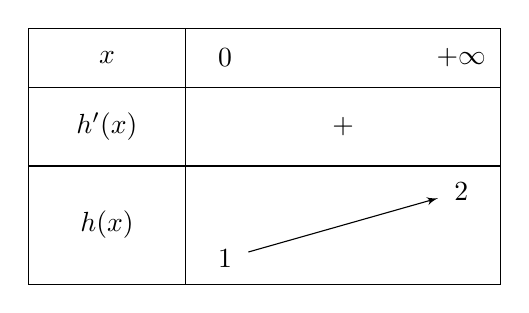
\begin{tikzpicture}
\tkzTabInit[]{
    $x$ /.75,
    $h'(x)$ /1,
    $h(x)$ /1.5
}{
    $0$,
    $+\infty$
}
\tkzTabLine{,+,}
\tkzTabVar{-/$1$,+/$2$}
\end{tikzpicture}
\end{center}
\end{multicols}

$g(x) = h(x) - x = \bfrac{1+2x}{1+x}-x = \bfrac{1+2x-x(1+x)}{1+x} = \bfrac{1+2x-x-x^2}{1+x} = \bfrac{1+x-x^2}{1+x}$

\noindent\textbf{\underline{Étude du signe de $x \mapsto -x^2+x+1$ :}}

Calcul du discriminant :  $\Delta = 1^2 - 4\times(-1)\times1 = 1+4 = 5$

$x_1 = \bfrac{-1-\sqrt{\Delta}}{-2} = \bfrac{1+\sqrt{5}}{2} = \varphi$
$\quad\quad\quad x_2 = \bfrac{-1+\sqrt{5}}{-2} = \bfrac{1-\sqrt{5}}{2} = -\bfrac{1}{\varphi}$

Vu que le coefficient du terme du plus haut degré est négatif, $x \mapsto -x^2+x+1$ est concave et s'annule en $x_1$ et $x_2$. Avec $x_1 \geq x^2$

\noindent\textbf{\underline{Étude du signe de $x \mapsto 1+x$ :}}

$x\mapsto1+x$ est positive pour $x\geq1$, s'annule en $x=-1$ et strictement croissante.

\noindent On en déduit le tableau de variation suivant sur $\R^*_+$ :

\begin{center}
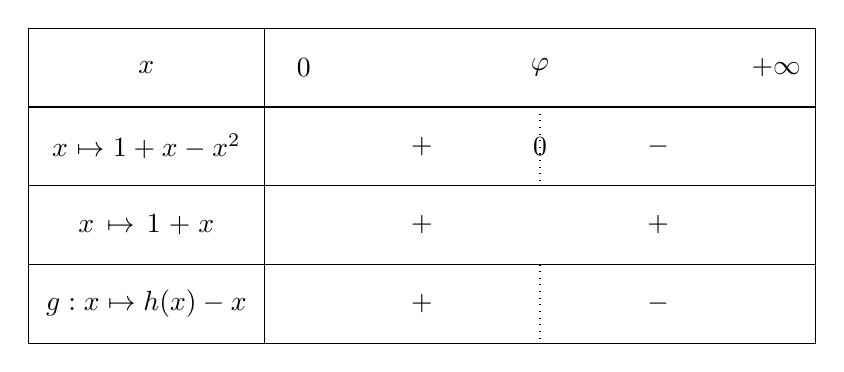
\begin{tikzpicture}
\tkzTabInit[lgt=3]{
    $x$ /1,
    $x\mapsto 1+x-x^2$ /1,
    $x\mapsto 1+x$ /1,
    $g: x \mapsto h(x) - x$ /1
}{
    $0$,
    $\varphi$,
    $+\infty$
}
\tkzTabLine{,+,z,-,}
\tkzTabLine{,+,,+,}
\tkzTabLine{,+,t,-,}
\end{tikzpicture}
\end{center}

\vspace{5px}
\textbf{2.c.}

Montrons par récurrence la propriété : $\forall n \in \N^*, \quad H_n: \text{"}U_{2n} \geq \varphi\text{"}$

\noindent\textbf{\underline{Initialisation :}}

Pour $n=1$ on a : $u_2 = f(u_1) = f(1) = 2$

$\varphi \approx 1.61$ donc $u_2 > \varphi$ d'où $H_1$ vraie.

\noindent\textbf{\underline{Hérédité :}}

On suppose $H_n$ vraie à un certain rang $n \in \N^*$. Montrons $H_{n+1}$ vraie.

D'après l'hypothèse de récurrence on a $u_{2n} > \varphi$ : 

\vspace{-12px}
\begin{flalign*}
u_{2n} &> \varphi &&\\
\text{Comme $h$ est croissante :} \Rightarrow h(u_{2n}) &> h(\varphi) &&\\
\Rightarrow u_{2(n+1)} &> h(\varphi) &&\\
\end{flalign*}

\vspace{-20px}
Calcul de $h(\varphi)$ :

\begin{flalign*}
h(\varphi) &= \bfrac{1+2\times\frac{1+\sqrt{5}}{2}}{1+\frac{1+\sqrt{5}}{2}} = \bfrac{2+\sqrt{5}}{\frac{3+\sqrt{5}}{2}} = \bfrac{2(2+\sqrt{5})}{3+\sqrt{5}} = \bfrac{2(2+\sqrt{5})}{3+\sqrt{5}}\times\bfrac{3-\sqrt{5}}{3-\sqrt{5}} &&\\
&= \bfrac{12-4\sqrt{5}+6\sqrt{5}-2\times5}{9-5} = \bfrac{2+2\sqrt{5}}{4} &&\\
&= \bfrac{1+\sqrt{5}}{2} = \varphi &&\\
\end{flalign*}

\vspace{-12px}

Ainsi, $u_{2(n+1)} > \varphi$, la relation est donc vrai au rang n+1.

\vspace{4px}
\noindent\textbf{\underline{Conclusion :}}

D'après le principe de récurrence, la propriété est vraie pour tout $n \in \mathbb{N}^*$. D'où : $\boxed{\forall n \in \N^*, \quad u_{2n} > \varphi}$

\vspace{5px}
\textbf{2.d.}

Pour montrer la décroissance de $(u_{2n})$ on étudie le signe de $u_{2(n+1)} - u_{2n}$

\begin{flalign*}
& u_{2(n+1)} - u_{2n} = h(u_{2n}) - u_{2n} = g(u_{2n}) &&\\
\end{flalign*}

Or on sait que g est négative sur $[\varphi, +\infty[$ et que $U_{2n} > \varphi$ don con peut dire que $g(u_{2n}) \leq 0$ et donc $(U_{2n})$ est décroissante.

\vspace{5px}
\textbf{2.e.}

On a $(u_{2n})$ décroissante et minoré par $\varphi$ donc $(u_{2n})$ converge vers un réel $l \in \R$.

On a $u_{2(n+1)} = h(u_{2n})$ et par passage à la limite $l = h(l)$

La limite de $(u_{2n})$ est solution de l'équation $l = h(l)$.

$l = \bfrac{1+2l}{1+l} \Leftrightarrow l(1+l) = 1+2l \Leftrightarrow l+l^2 = 1+2l \Leftrightarrow l^2-l-1 = 0$

Calcul du discriminant : $\Delta = (-1)^2 - 4\times1\times(-1) = 1+4 = 5$

$l_1 = \bfrac{-(-1)-\sqrt{5}}{2} = \bfrac{1-\sqrt{5}}{2} = - \bfrac{1}{\varphi}$
$\quad\quad\quad\quad l_2 = \bfrac{-(-1) + \sqrt{5}}{2} = \bfrac{1+\sqrt{5}}{2} = \varphi$

On sait que la suite $(u_{2n}$ est minoré par $\varphi$ donc la limite $l$ est positive. On choisi $l_2 = \varphi$ comme solution.

\vspace{15px}
\noindent Ainsi :

\vspace{-30px}
\[\boxed{u_{2n} \longrightarrow \varphi}\]

\vspace{10px}
\textbf{2.f.}

$u_{2(n+1)+1} = u_{2n+3} = f(u_{2n+2}) = f(f(u_{2n+1})) = h(u_{2n+1})$

Donc $u_{2(n+1)+1} = h(u_{2n+1})$, la suite $(u_{2n+1}$ est récurrente par la fonction $h$.

Montrons par récurrence la propriété : $\forall n \in \N, \quad P_n: \text{"}0  < U_{2n+1} \leq \varphi \text{"}$

\noindent\textbf{\underline{Initialisation :}}

Pour $n=0$ on a : $u_1 = 1$, et $0 < 1 \leq \varphi$ donc $P_0$ est vraie.

\noindent\textbf{\underline{Hérédité :}}

On suppose $P_n$ vraie à un certain rang $n \in \N^*$. Montrons $P_{n+1}$ vraie.

D'après l'hypothèse de récurrence on a $0 < u_{2n+1} \leq \varphi$ : 

\vspace{-12px}
\begin{flalign*}
0 < &u_{2n+1} \leq \varphi &&\\
\text{Comme $h$ est croissante :} \Rightarrow \; 1 < h(&u_{2n+1}) \leq h(\varphi) &&\\
\text{D'après la question précédente :} \Rightarrow \; 1 < &u_{2(n+1)+1} \leq \varphi &&\\
\end{flalign*}

On note que $h$ est prolongeable par continuité en $x = 0$ et donc que $h(0) = 1$

Ainsi $P_{n+1}$ est vraie.

\vspace{4px}
\noindent\textbf{\underline{Conclusion :}}

D'après le principe de récurrence, la propriété est vraie pour tout $n \in \mathbb{N}$. D'où : $\forall n \in \N, \quad 0 < u_{2n+1} \leq \varphi$

Ainsi, $\forall n \in \N, u_{2n+1} \in ]0, \varphi]$

\noindent On veut ensuite montrer $(u_{2n+1})$ croissante, montrons : $u_{2(n+1)+1} \geq u_{2n+1}$

On pose $p(n) = u_{2(n+1)+1} - u_{2n+1} = h(u_{2n+1}-u_{2n+1} = g(u_{2n+1})$. Or on sait que $0 < u_{2n+1} \leq \varphi$. Donc d'après le tableau de variation dressé à la question 2.b, on a $\forall n \in \N, \; p(n) \geq 0$. D'où, $(u_{2n+1})$ croissante.

La suite $(u_{2n+1})$ est majoré et croissante c'est donc qu'elle admet une limite noté $l' \in \R$ en $+\infty$, par passage à la limite on obtient la même équation du second degré. 

$u_{2(n+1)+1} = h(u_{2n+1} \Leftrightarrow l' = h(l) \Leftrightarrow l'^2-l'-1 = 0$

On choisit la racine positive et on obtient que : $l' = \varphi$. Ainsi $(u_{2n+1})$, converge vers $\varphi$

\begin{center}
\boxed{$(u_{2n+1})$ est croissante, converge vers $\varphi$ et $\forall n \in \N, \; u_{2n+1} \in ]0, \varphi]$}
\end{center}

\vspace{5px}
\textbf{2.g.}

$(u_{2n})$ et $(u_{2n+1})$ sont deux suites extraites qui contiennent respectivement les termes pairs et les termes impairs. Ces deux suites admettent la même limite $\varphi$. Donc $(u_n)$ admet cette même limite.

\vspace{15px}
\noindent Ainsi :
\vspace{-15px}
\[\boxed{u_n \longrightarrow \varphi}\]

\vspace{10px}
\textbf{2.h.}

$v_n = \bfrac{F_{n+1}}{F_n}$\quad
Donc : $v_{n+1} = \bfrac{F_{n+1+1}}{F_{n+1}} = \bfrac{F_{n+2}}{F_{n+1}} = \bfrac{F_{n+1} + F_n}{F_{n+1}} = 1 + \bfrac{F_n}{F_{n+1}} = f(\bfrac{F_{n+1}}{F_n}) = f(v_n)$

Ainsi vu que $v_n$ est définit avec $n \in \N^*$, $v_1 = \frac{1}{1} = 1$ et que $v_{n+1} = f(v_n)$, on déduit que $\forall n \in \N^*, \; v_n = u_n$. Les deux suite sont égales donc elles admettent la même limite $\varphi$

\vspace{15px}
\noindent Ainsi :
\vspace{-15px}
\[\boxed{v_n \longrightarrow \varphi}\]

\vspace{15px}

\textbf{3.a.}

Montrons par récurrence la propriété : $\forall n \in \N, \quad Q_n: \text{"} F_{n+1}^2-F_{n+2}F_n = (-1)^n \text{"}$

\noindent\textbf{\underline{Initialisation :}}

Pour $n=0$ on a d'une part $F_{1}^2 - F_{2}F_0 = 1 - 0 = 1$ et d'une autre part $(-1)^0 = 1$. Donc $Q_0$ est vraie.

\noindent\textbf{\underline{Hérédité :}}

On suppose $Q_n$ vraie à un certain rang $n \in \N^*$. Montrons $Q_{n+1}$ vraie.

D'après l'hypothèse de récurrence : 

\vspace{-10px}
\begin{flalign*}
& F_{n+1}^2 - F_{n+2}F_n = (-1)^n &&\\
&\implies (-1)(F_{n+1}^2 - F_{n+2}F_n) = (-1)^{n+1} &&\\
&\implies -F_{n+1}^2+(F_{n+1} + F_{n})F_n = (-1)^{n+1} &&\\
&\implies -F_{n+1}^2+F_n\times F_{n+1} + F_n^2 = (-1)^{n+1} &&\\
&\implies F_{n+1}(F_n-F_{n+1}) + F_n^2 = (-1)^{n+1} &&\\
&\implies F_{n+1}^2 + 2F_{n+1}F_n + F_n^2 - (F_{n+1}^2 + F_{n+2}F_{n+1}) = (-1)^{n+1} &&\\
&\implies (F_{n+1} + F_n)^2 - (F_{n+1} + F_{n+2})F_{n+1} = (-1)^{n+1} &&\\
&\implies F_{n+2}^2 - F_{n+3}F_{n+1} = (-1)^{n+1}
\end{flalign*}

\vspace{4px}
Ainsi $Q_{n+1}$ est vraie.

\vspace{4px}
\noindent\textbf{\underline{Conclusion :}}

D'après le principe de récurrence, la propriété est vraie pour tout $n \in \mathbb{N}$.

\vspace{15px}
\noindent Par conséquence :
\vspace{-15px}
\[\boxed{\forall n \in \N, \quad F_{n+1}^2 - F_{n+2}F_n = (-1)^n}\]
\vspace{10px}

\textbf{3.b.}

\noindent $v_{n+1} - v_n = \bfrac{F_{n+1+1}}{F_{n+1}} - \bfrac{F_{n+1}}{F_n} = \bfrac{F_{n+2}}{F_{n+1}} - \bfrac{F_{n+1}}{F_{n}} = \bfrac{F_{n+2}F_n - F_{n+1}^2}{F_{n+1}F_n} = \bfrac{(F_n+F_{n+1})F_n - F_{n+1}^2}{F_{n+1}F_n}$

\noindent D'après la question précédente : $v_{n+1} - v_n = \bfrac{F_n^2 + F_{n+1}F_n - F_{n+1}^2}{F_{n+1}F_n} = \bfrac{F_n^2 + F_{n+3}F_{n+1}}{F_{n+1}F_n} = \bfrac{(-1)^{n+1}}{F_{n+1}F_n}$

\vspace{15px}
\noindent Donc :
\vspace{-15px}
\[\boxed{\forall n \in \N^*, \quad v_{n+1} - v_n = \bfrac{(-1)^{n+1}}{F_n F_{n+1}}} \]
\vspace{10px}

\textbf{3.c.}

\quad

\quad

\quad

\quad

\quad
\quad

\quad

\quad

\quad

\quad
\quad

\quad

\quad

\quad

\quad
\quad

\quad

\quad

\quad

\quad
\quad

\quad

\quad

\quad

\quad

\quad

\quad

\quad

\quad

\quad

\textbf{3.d.} A la fin du programme, la variable $F$ contient le n-ième terme de la suite $(F_n)$ et la variable $FF$ contient le (n-1)-ième terme de la même suite.
La variable $x$ vérifie $x = \bfrac{F_n}{F_{n-1}}$ et $y = \bfrac{\frac{1}{F_n}}{F_{n-1}} $
X et Y peuvent être interprétés comme les coordonnées d'un point associé à un terme de la suite $(F_n)$ sur un graphique, à mesure que l'indice n grandit, la coordonnée $x$ se rapproche de 0 alors que $y$ tend vers $\varphi$, c'est une approximation du nombre d'or.

\textbf{4.a.}
%\begin{cases} n/2, & \mbox{if } n\mbox{ is even} \\ 3n+1, & \mbox{if } n\mbox{ is odd} \end{cases}
On cherche l'expression explicite d'une suite récurrente linéaire d'ordre 2.

L'équation caractéristique de $(F_n)$ est : $-x^2+x+1 = 0$

Calcul du discriminant : $\Delta = 1^2-4(-1)\times1 = 1+4 = 5$

On a donc deux racines : $x_1 = \varphi$ et $x_2 = -\bfrac{1}{\varphi}$

L'expression explicite de $F_n$ est de la forme :
$F_n = \alpha \cdot x_1^n + \beta \cdot x_2^n$. Avec $\alpha, \beta \in \R$. 

On a donc : $F_n = \alpha \cdot \varphi^n + \beta \cdot \big(-\frac{1}{\varphi}\big)^n$.

Cherchons $\alpha$ et $\beta$ :

\[
\begin{cases}
F_0 = 0 = \alpha + \beta \\
F_1 = 1 = \alpha\cdot\varphi +\beta\cdot\big(-\frac{1}{\varphi}\big)
\end{cases}
\Leftrightarrow
\begin{cases}
\alpha = -\beta \\
1 = -\beta\cdot\frac{1+\sqrt{5}}{2} + \beta\cdot\frac{1-\qrt{5}}{2}
\end{cases}
\Leftrightarrow
\begin{cases}
\alpha = -\beta \\
1 = \beta(\frac{1-\sqrt{5}}{2}-\frac{1+\sqrt{5}}{2})
\end{cases}
\]
\vspacem
\[
\Leftrightarrow
\begin{cases}
\alpha = -\beta \\
\beta = \bfrac{1}{\frac{1-\sqrt{5}}{2} + \frac{1+\sqrt{5}}{2}} = \bfrac{2}{-2\sqrt{5}}
\end{cases}
\Leftrightarrow
\begin{cases}
\alpha = \frac{1}{\sqrt{5}} \\
\beta = -\frac{1}{\sqrt{5}}
\end{cases}
\]

\vspace{2px}
\noindent Donc on obtient l'expression explicite de $(F_n)$ :

$F_n = \bfrac{1}{\sqrt{5}}\varphi^n + \bfrac{1}{\sqrt{5}}\cdot\bfrac{1}{\varphi} = \bfrac{1}{\sqrt{5}}\Bigg(\varphi^n+\bigg(\frac{-1}{\varphi}\bigg)^n\Bigg)$

On note $\varphi' = -\bfrac{1}{\varphi}$

\vspace{15px}
\noindent Donc :
\vspace{-15px}
\[\boxed{\forall n \in \N, \quad F_{n}={\frac {1}{\sqrt {5}}}(\varphi ^{n}-\varphi '^{n})} \]
\vspace{10px}

\textbf{4.b.}

Montrer $F_n \underset{+\infty}{\sim} \bfrac{\sqrt{5}}{5}\varphi^n $ reviens à montrer que $\bfrac{F_n - \frac{\sqrt{5}}{5}\varphi^n}{\frac{\sqrt{5}}{5}\varphi^n} \underset{+\infty}{\longrightarrow} 0$

$\bfrac{F_n - \frac{\sqrt{5}}{5}\varphi^n}{\frac{\sqrt{5}}{5}\varphi^n} = \bfrac{\frac{1}{\sqrt{5}}(\varphi^n-\varphi'^n)}{\frac{\sqrt{5}}{5}} - 1 = \bfrac{5}{\varphi^n\sqrt{5}} \cdot \bfrac{1}{\sqrt{5}}(\varphi^n - \varphi'^n) - 1 = \bfrac{1}{\varphi^n}(\varphi^n - \varphi'^n) - 1 = - \bfrac{\varphi'^n}{\varphi^n}$

Vu que $|\varphi'| < 1$, $\varphi'^n \longrightarrow 0$ et vu que $|\varphi| > 1$, $\varphi^n \longrightarrow +\infty$. Ainsi $- \bfrac{\varphi'^n}{\varphi^n} \longrightarrow 0$

\vspace{15px}
\noindent Donc :
\vspace{-15px}
\[\boxed{F_n \underset{+\infty}{\sim} \bfrac{\sqrt{5}}{5}\varphi^n} \]
\vspace{10px}

On sait que $F_n \underset{+\infty}{\sim} \bfrac{\sqrt{5}}{5}\varphi^n$ et que $F_{n+1} \underset{+\infty}{\sim} \bfrac{\sqrt{5}}{5}\varphi^{n+1}$.

On obtient donc :  $\bfrac{F_{n+1}}{F_n} \underset{+\infty}{\sim} \bfrac{\frac{\sqrt{5}}{5}\cdot\varphi^{n+1}}{\frac{\sqrt{5}}{5}\cdot\varphi^{n}} \underset{+\infty}{\sim} \varphi$

\vspace{15px}
\noindent Ainsi :
\vspace{-15px}
\[\boxed{\bfrac{F_{n+1}}{F_n} \longrightarrow +\infty} \]

\end{document}

